\subsection{Division of Tasks}
WRITTEN BY DENNIS 
How did you split the workload? Were individual team members assigned to be responsible for specific parts of the project?

Tasks have been iteratively delegated to members 
We have chosen tasks independent from time consumption
Divide and conquer 
\begin{itemize}
	\item Workload has both joint and individual 
	\item Initially split work in sections and components 
	\item Subsections were individual 
	\item Group work: split in subsections 
	\item Iterative distribution, qualified guess, too big workload (Waterfall) 
	\item Tasks divided in topics or code packages 
\end{itemize}

RAD Example: split into sections of Introduction, Current System, Proposed System and graphical content (scenario, use case, object model, dynamic model)

Work load is based on the time spent for each task 

Things that involve decisions on the future implementation of the program have been worked on in collaboration by all members (e.g. design goals)


\textbf{NEED TABLE}

% RAD TIME TABLE 
\begin{figure}[H]
	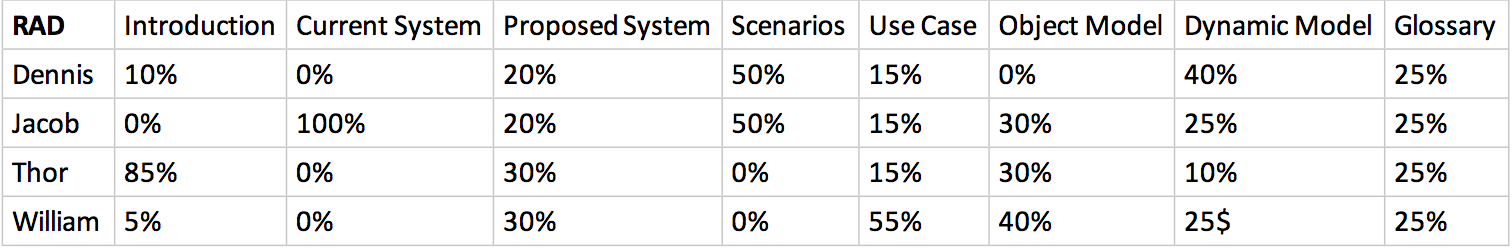
\includegraphics{radtimetable}
	\caption{RAD Work Distribution}
	\label{fig:rad}
\end{figure}

% SDD TIME TABLE 
\begin{figure}[H]
	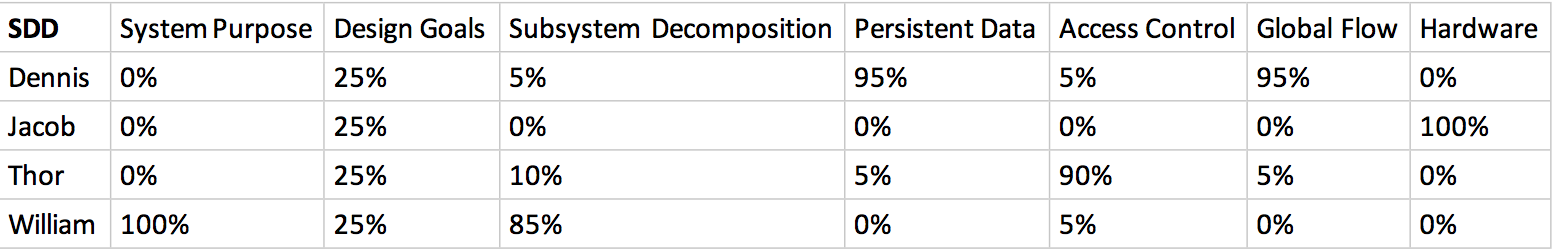
\includegraphics{sddtimetable}
	\caption{SDD Work Distribution}
	\label{fig:sdd}
\end{figure}

% Code Skeleton TIME TABLE 
\begin{figure}[H]
	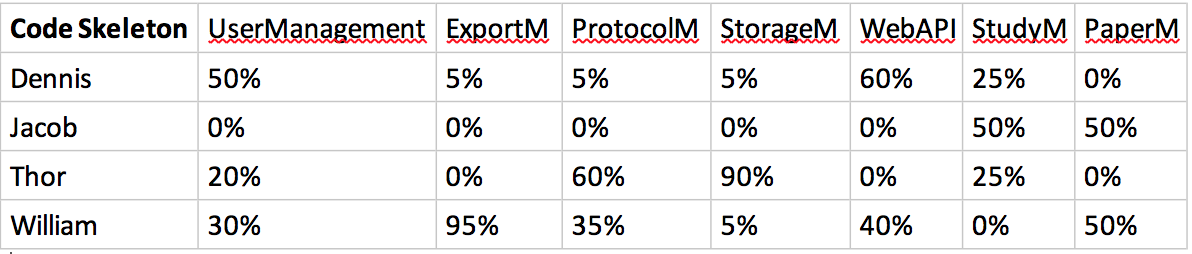
\includegraphics{image/skeletontimetable}
	\caption{Code Skeleton Work Distribution}
	\label{fig:codeskeleton} % To use write \ref{fig:codeskeleton}
\end{figure}
